\clearpage
\chapter{Study Guide 6}

\section{Matrices}
\horizontalline{0}{0}

\begin{center}
    \large{\textbf{Study Guide Instructions}}
\end{center}

\horizontalline{-1}{0}

\begin{itemize}
    \item Submit your work in Gradescope as a PDF - you will identify where your “questions are.”
    \item Identify the question number as you submit.  Since we grade "blind" if the questions are NOT identified, the work WILL NOT BE GRADED and a 0 will be recorded. Always leave enough time to 
    identify the questions when submitting.
    \item One section per page (if a page or less) - We prefer to grade the main solution in a single page, extra work can be included on the following page.
    \item Long instructions may be removed to fit on a single page.
    \item \textbf{Do not start a new question in the middle of a page.}
    \item Solutions to book questions are provided for reference.
    \item You may NOT submit given solutions - this includes minor modifications - as your own.
    \item Solutions that do not show individual engagement with the solutions will be marked as no credit and can be considered a violation of honor code.
    \item If you use the given solutions you must reference or explain how you used them, in particular...
\end{itemize}

\horizontalline{-1}{0}

\begin{center}
    \large{\textbf{Method Selection}}
\end{center}

\horizontalline{-1}{0}

\textbf{For full credit,  EACH book exercise in the Study Guides must use one or more of the following methods and FOR EACH QUESTION.  Identify the number the method by number to ensure full credit.}

\begin{itemize}
    \item \textbf{Method 1} - Provide original examples which demonstrate the ideas of the exercise in addition to your solution.
    \item \textbf{Method 2} - Include and discuss the specific topics needed from the chapter and how they relate to the question.
    \item \textbf{Method 3} - Include original Python code, of reasonable length (as screenshot or text)  to show how the topic or concept was explored.
    \item \textbf{Method 4} - Expand the given solution in a significant way, with additional steps and comments. All steps are justified. This is a good method for a proof for which you are only given a basic outline.
    \item \textbf{Method 5} - Attempt the exercise without looking at the solution and then the solution is used to check work. Words are used to describe the results.
    \item \textbf{Method 6} - Provide an analysis of the strategies used to understand the exercise, describing in detail what was challenging, who helped you or what resources were used. The process of understanding is
    described.
\end{itemize}

% Problem 1
\begin{problem}{Problem 1}
    \begin{statement}{Problem Statement}
        Pick a section of Chapter 6 to annotate.
    \end{statement}

    For annotations this week, I have chosen to annotate section 6.4 of VMLS. The annotations for this problem can be seen on the following page.

    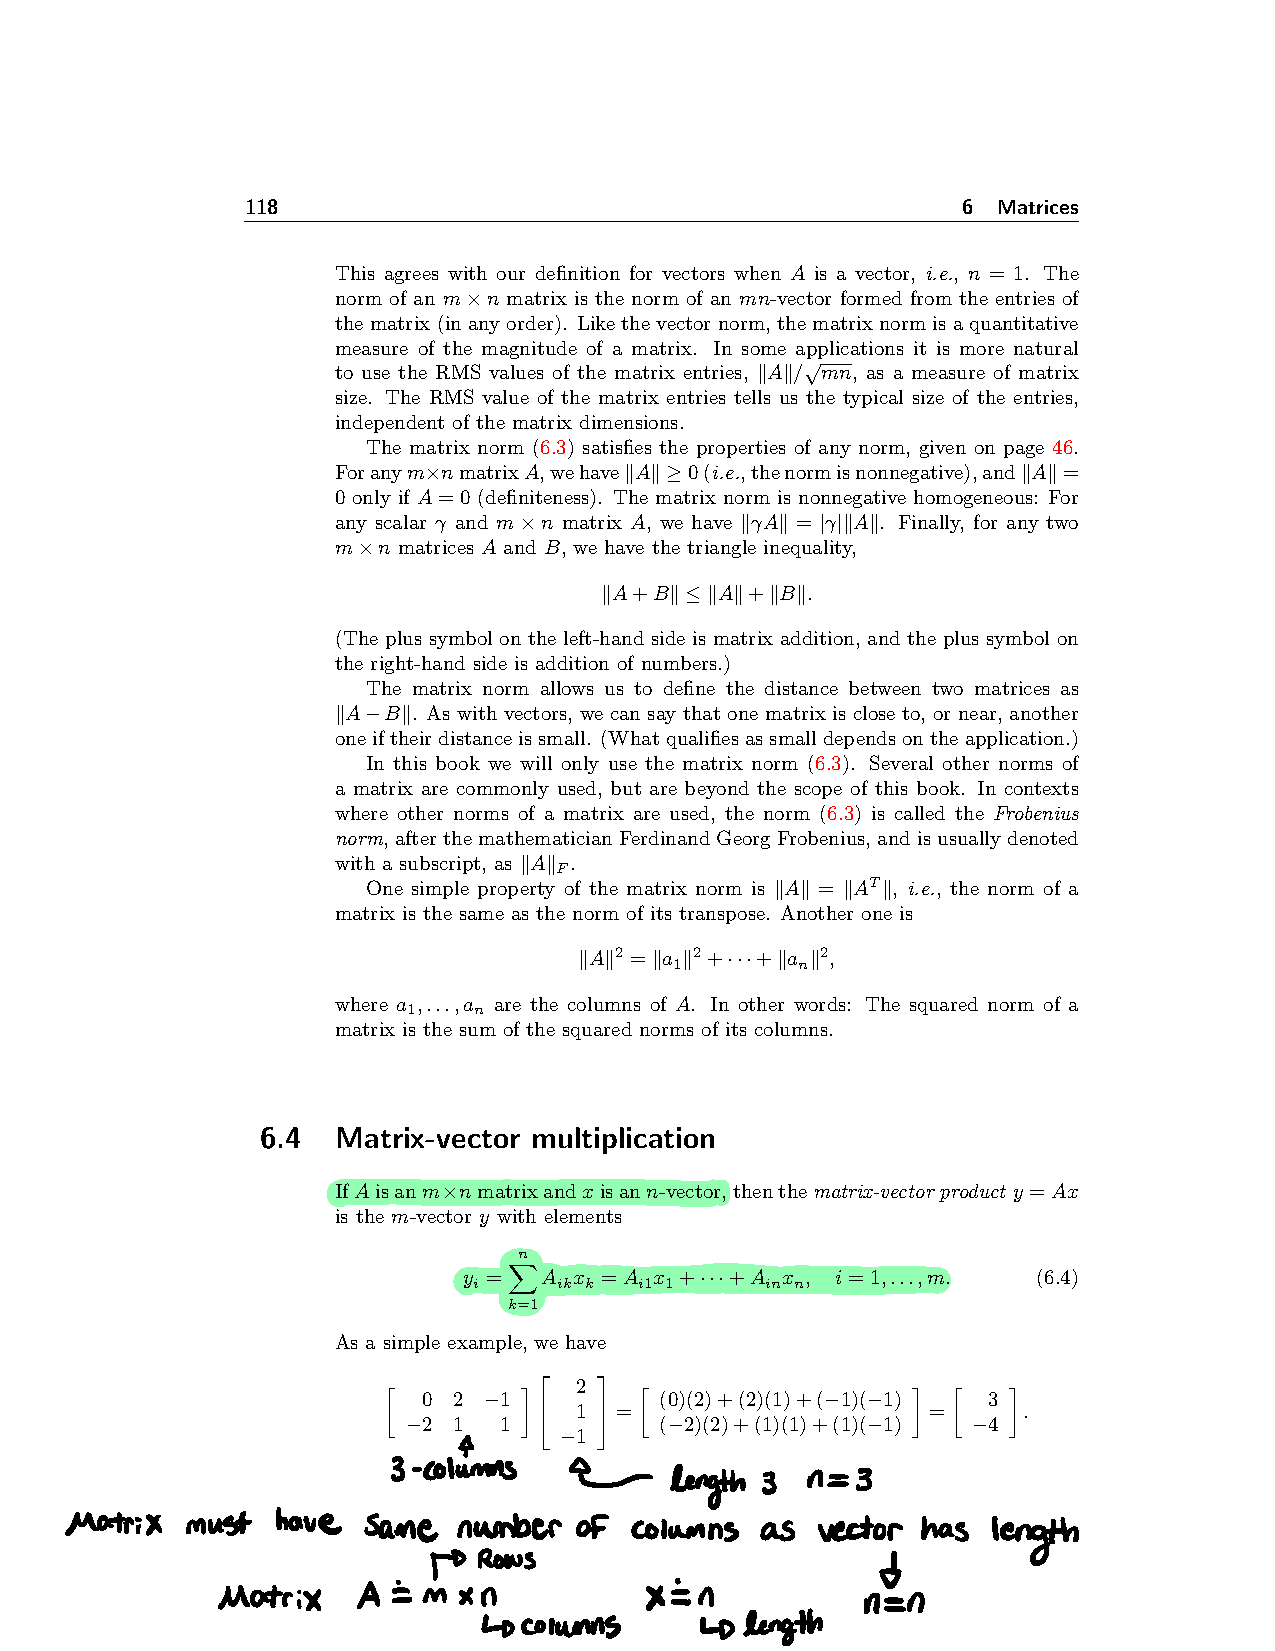
\includepdf[pages={-}, pagecommand={\thispagestyle{fancy}}, width=\paperwidth, offset=0 0]{./PDF/Annotations.pdf}
\end{problem}

% Problem 1 Summary
\begin{summary}{Problem 1 Summary}
    \begin{statement}{Procedure}
        \begin{itemize}
            \item Annotate a chapter from VMLS and highlight important concepts from the section.
        \end{itemize}
    \end{statement}
    \begin{statement}{Key Concepts}
        \begin{itemize}
            \item This section highlights the aspects involving matrix vector multiplication.
            \item In order to perform matrix / vector multiplication the number of columns in the matrix must match the number of rows in the vector.
            \begin{itemize}
                \item Namely, $n$ must be equal in $(m \times n) \times (n \times m)$. First value is the number of rows and the second is columns.
            \end{itemize}
        \end{itemize}
    \end{statement}
    \begin{statement}{Variations}
        \begin{itemize}
            \item Since this problem involves annotating a section, the only variation of this problem could involve annotating another section.
            \begin{itemize}
                \item We would then comment on the sections just like we did in the original problem.
            \end{itemize}
        \end{itemize}
    \end{statement}
\end{summary}

% Problem 2
\begin{problem}{Problem 2}
    \begin{statement}{Problem Statement}
        Solve and explain the solution to 6.3  here in your own words. (Since you are given a solution, you will be graded on your ability to explain). \vspace*{1em}

        \noindent \textbf{Original Question} \vspace*{1em}

        \textit{Block matrix.} Assuming the matrix

        \begin{equation*}
            K = 
            \begin{bmatrix}
                I & A^{T} \\
                A & 0 \\
            \end{bmatrix}
        \end{equation*}
        makes sense, which of the following statements must be true? (`Must be true' means that it follows with no additional assumptions.)

        \begin{enumerate}[label = (\alph*)]
            \item $K$ is square.
            \item $A$ is square or wide.
            \item $K$ is symmetric, \textit{i.e.,} $K^{T} = K$.
            \item The identity and zero submatrices in $K$ have the same dimensions.
            \item The zero submatrix is square.
        \end{enumerate}
    \end{statement}

    \begin{Highlight}[Solution - Part (a)]
        For this problem I will be using \textbf{Method 4}. \vspace*{1em}

        \noindent \textbf{VMLS Solution:}

        \begin{enumerate}[label = (\alph*)]
            \item Must be true. $K$ is $(m + n) \times (m + n)$.
        \end{enumerate}

        \noindent \textbf{Explanation:}

        \begin{enumerate}[label = (\alph*)]
            \item We know from the properties of matrices we can write the dimension of a matrix as $m \times n$. We know that identity matrices are square ($m \times m$). Zero matrices are matrices 
            where every entry is a 0 so it can be of an arbitrary size, such as ($m \times n$). As for the matrix $A$ it can be of an arbitrary size such as ($m \times n$). Expanding this for matrix $K$ 
            we can then see that the matrix is consisted of submatrices with the following dimensions

            \begin{equation}
                K = 
                \begin{bmatrix}
                    n \times n & n \times m \\
                    m \times n & m \times m \\
                \end{bmatrix}.
            \end{equation}
            For a matrix to be square, it must have the same number as rows as columns. From the refined definition of $K$ in (1), we see that the dimension of $K$ is then

            \begin{equation}
                (n + m) \times (n + m).
            \end{equation}
            Since, from (2) we see that $K$ indeed has the same number of rows as columns, we know that $K$ is indeed \textbf{square}. This statement \textbf{must be true}.
        \end{enumerate}
    \end{Highlight}

    \begin{Highlight}[Solution - Part (b)]
        For this problem I will be using \textbf{Method 4}. \vspace*{1em}

        \noindent \textbf{VMLS Solution:}

        \begin{enumerate}[label = (\alph*), start = 2]
            \item Might not be true. A could be tall.
        \end{enumerate}

        \noindent \textbf{Explanation:}

        \begin{enumerate}[label = (\alph*), start = 2]
            \item Since $A$ is of an arbitrary size, it is completely possible that $A$ could have a larger value for $m$ than it does for $n$. Because of this, any of the possible
            matrix descriptions are valid:

            \begin{itemize}
                \item \textbf{Square:} $m \times n$ where $n = m$
                \item \textbf{Tall:} $m \times n$ where $m > n$
                \item \textbf{Wide:} $m \times n$ where $m < n$
            \end{itemize}
            Because of this reality, the statement \textbf{might not be true}.
        \end{enumerate}
    \end{Highlight}

    \begin{Highlight}[Solution - Part (c)]
        For this problem I will be using \textbf{Method 4}. \vspace*{1em}

        \noindent \textbf{VMLS Solution:}

        \begin{enumerate}[label = (\alph*), start = 3]
            \item Must be true. Using the block transpose formula on $K$, you get $K$ back again.
        \end{enumerate}

        \noindent \textbf{Explanation:}

        \begin{enumerate}[label = (\alph*), start = 3]
            \item For a matrix to be considered symmetric, it must follow that $A = A^{T}$ where $A_{ij} = A_{ji}$ for all values of $i$ and $j$. If we transpose the block matrix $K$ we see
            
            \begin{equation}
                K^{T} = 
                \begin{bmatrix}
                    I & A^{T} \\
                    A & 0 \\
                \end{bmatrix}^{T}
                = 
                \begin{bmatrix}
                    I^{T} & A^{T} \\
                    A & 0^{T} \\
                \end{bmatrix}
                = 
                \begin{bmatrix}
                    I & A^{T} \\
                    A & 0 \\
                \end{bmatrix}
                = K.
            \end{equation}
            In order for $K$ to be indeed square, we require that $0^{T} = 0$. Because of this we can see that the transposes are indeed equal and thus $K$ is symmetric. Therefore the statement 
            \textbf{must be true}.
        \end{enumerate}
    \end{Highlight}

    \begin{Highlight}[Solution - Part (d)]
        For this problem I will be using \textbf{Method 4}. \vspace*{1em}

        \noindent \textbf{VMLS Solution:}

        \begin{enumerate}[label = (\alph*), start = 4]
            \item Might not be true. They are $n \times n$ and $m \times m$, respectively, and we don’t need to have $m = n$.
        \end{enumerate}

        \noindent \textbf{Explanation:}

        \begin{enumerate}[label = (\alph*), start = 4]
            \item We know from part (a) that in this example, both the identity and zero matrices are square. This of course means that $I = n \times n$ and $0 = m \times m$. This follows because
            in order for $K$ to be square, 0 must have the same number of rows $A$, so this means that $0 = m \times m$. As for the identity, $I$ must have the same number of rows as $A^{T}$, so
            $I = n \times n$. This then implies that it is not a necessary condition that $n = m$ and thus $I$ and 0 don't necessarily have to be of the same dimension. Therefore the statement
            \textbf{might not be true}.
        \end{enumerate}
    \end{Highlight}

    \begin{Highlight}[Solution - Part (e)]
        For this problem I will be using \textbf{Method 4}. \vspace*{1em}

        \noindent \textbf{VMLS Solution:}

        \begin{enumerate}[label = (\alph*), start = 5]
            \item Must be true. The zero submatrix has dimensions $m \times m$.
        \end{enumerate}

        \noindent \textbf{Explanation:}

        \begin{enumerate}[label = (\alph*), start = 5]
            \item We have pretty much shown this in the previous parts. In order for $K$ to be square, it must follow that the 0 submatrix is square in order for it to be symmetric. Because of this
            we know that $0 = m \times m$ and is indeed square. Therefore the statement \textbf{must be true}.
        \end{enumerate}
    \end{Highlight}
\end{problem}

% Problem 2 Summary
\begin{summary}{Problem 2 Summary}
    \begin{statement}{Procedure}
        \begin{itemize}
            \item For part (a), add up the number of rows and columns to determine the size of the matrix.
            \item For part (b), reason that because the matrix is of an arbitrary size it is possible that it could be tall.
            \item For part (c), because of the nature of $K$ being square, we can reason that it is also symmetric.
            \item For part (d), reason that because the identity matrix is square, it is not necessarily true that the submatrix $A$ is going to be of the same dimension.
            \item For part (e), reason that because of the dimensions of the identity and $A$ matrix and the shape of $K$ that the zero matrix must be square.
        \end{itemize}
    \end{statement}
    \begin{statement}{Key Concepts}
        \begin{itemize}
            \item \textbf{Squareness of Matrix $K$:} The matrix $K$ is determined to be square based on the arrangement and dimensions of its submatrices.
            \item \textbf{Matrix $A$ Can Be Square or Wide:} The matrix $A$ can have arbitrary dimensions, meaning it could be square, tall, or wide.
            \item \textbf{Symmetry of Matrix $K$:} The symmetry of the matrix $K$ is deduced by applying the block transpose formula, leading to the conclusion that $K^{T} = K$.
            \item \textbf{Dimensions of Identity and Zero Matrices:} The identity and zero submatrices in $K$ do not necessarily have the same dimensions.
            \item \textbf{Zero Submatrix Being Square:} The zero submatrix in $K$ is shown to be square to maintain the overall square structure of $K$.
            \item \textbf{Block Matrix Analysis:}
            \begin{itemize}
                \item The problem involves analyzing a block matrix $K$ and determining the truth of several statements about its properties.
                \item The matrix $K$ is assumed to be in a block form involving an identity matrix $I$, a zero matrix, and a matrix $A$ along with its transpose $A^{T}$.
            \end{itemize}
        \end{itemize}
    \end{statement}
    \begin{statement}{Variations}
        \begin{itemize}
            \item We could be given a different matrix with submatrices to examine.
            \begin{itemize}
                \item We would then use the same logic of determining what the sizes and shapes of the matrices are.
            \end{itemize}
        \end{itemize}
    \end{statement}
\end{summary}

% Problem 3
\begin{problem}{Problem 3}
    \begin{statement}{Problem Statement}
        Solve and Explain the solution to 6.9  here in your own words. (Since you are given a solution, you will be graded on your ability to explain). \vspace*{1em}

        \noindent \textbf{Original Question} \vspace*{1em}

        Multiple channel marketing campaign. Potential customers are divided into $m$ market segments, which are groups of customers with similar demographics, e.g., college educated women aged 25–29. 
        A company markets its products by purchasing advertising in a set of $n$ channels, i.e., specific TV or radio shows, magazines, web sites, blogs, direct mail, and so on. The ability of each 
        channel to deliver impressions or views by potential customers is characterized by the reach matrix, the $m \times n$ matrix $R$, where $R_{ij}$ is the number of views of customers in segment $i$ 
        for each dollar spent on channel $j$. (We assume that the total number of views in each market segment is the sum of the views from each channel, and that the views from each channel scale 
        linearly with spending.) The $n$-vector $c$ will denote the company's purchases of advertising, in dollars, in the $n$ channels. The $m$-vector $v$ gives the total number of impressions in the 
        $m$ market segments due to the advertising in all channels. Finally, we introduce the $m$-vector $a$, where $a_{i}$ gives the profit in dollars per impression in market segment $i$. The entries 
        of $R, c, v,$ and $a$ are all nonnegative.

        \begin{enumerate}[label = (\alph*)]
            \item Express the total amount of money the company spends on advertising using vector/matrix notation.
            \item Express $v$ using vector/matrix notation, in terms of the other vectors and matrices.
            \item Express the total profit from all market segments using vector/matrix notation.
            \item How would you find the single channel most effective at reaching market segment 3, in terms of impressions per dollar spent?
            \item What does it mean if $R_{35}$ is very small (compared to other entries of $R$)?
        \end{enumerate}
    \end{statement}

    \begin{Highlight}[Solution - Part (a)]
        For this problem I will be using \textbf{Method 4}. \vspace*{1em}

        \noindent \textbf{VMLS Solution:}

        \begin{enumerate}[label = (\alph*)]
            \item $1^{T}c$. The company's purchases in advertising for the $n$ channels is given by $c$, so summing up the entries of $c$ gives the total amount of money the company spends across 
            all channels.
        \end{enumerate}

        \noindent \textbf{Explanation:}

        \begin{enumerate}[label = (\alph*)]
            \item In order to correctly represent the amount of money that the company spends on advertising for these channels we need a scalar value. In the context of vector notation, to generate
            a scalar value we would use an inner product. Since we do not want to alter the cost of advertising for a specific channel, we would want to multiply that cost for the given channel with 1.
            In the context of vectors, this would mean an inner product of length $n$ for the $1$ vector with the cost vector $c$. Namely,

            \setcounter{equation}{0}
            \begin{equation}
                C = 1^{T}c
            \end{equation}
            where $C$ is the total cost of advertising. We are effectively summing up the cost of advertising the company spends for all channels.
        \end{enumerate}
    \end{Highlight}

    \begin{Highlight}[Solution - Part (b)]
        For this problem I will be using \textbf{Method 4}. \vspace*{1em}

        \noindent \textbf{VMLS Solution:}

        \begin{enumerate}[label = (\alph*), start = 2]
            \item $v = Rc$. To find the total number of impressions $v_{i}$ in the $i$th market segment, we need to sum up the impressions from each channel, which is given by an inner product of the 
            $i$th row of $R$ and the amounts $c$ spent on advertising per channel.
        \end{enumerate}

        \noindent \textbf{Explanation:}

        \begin{enumerate}[label = (\alph*), start = 2]
            \item Because we want a vector representation for $v$, this most likely means that we need to multiply a matrix with a vector. In this context, we know that $R$ is a matrix and $c$ is a 
            vector. Since $R$ represents the number of views of customers on a segment $i$ for each dollar spent on channel $j$, we would want to multiply the row of $R$ with the vector $c$ that represents
            the cost the company spent on advertising for a given channel. Piecing this together we have the expression

            \begin{equation}
                v = Rc.
            \end{equation}
            Because of the nature of matrix/ vector multiplication, each entry in $v$ will denote the number of impressions for each segment across all channels.
        \end{enumerate}
    \end{Highlight}

    \begin{Highlight}[Solution - Part (c)]
        For this problem I will be using \textbf{Method 4}. \vspace*{1em}

        \noindent \textbf{VMLS Solution:}

        \begin{enumerate}[label = (\alph*), start = 3]
            \item $a^{T}v = a^{T}Rc$. The total profit is the sum of the profits from each market segment, which is the product of the number of impressions for that segment $v_{i}$ and the profit 
            per impression for that segment $a_{i}$. The total profit is the sum $\sum_{i} a_{i}v_{i} = a^{T}v$. Substituting $v = Rc$ gives $a^{T}v = a^{T}Rc$.
        \end{enumerate}

        \noindent \textbf{Explanation:}

        \begin{enumerate}[label = (\alph*), start = 3]
            \item Since we know that $v$ represents the total number of impressions across all segments from all channels, we would want to sum the total profit from each segment to get the final 
            profit across all segments. We would then need to multiply the profit per impression for each segment with the total number of impressions for the given segment. This is screaming for a
            inner product of two vectors. So, we then take the inner product of $a$ (the profit in dollars per impressions for a given segment) with that of the $v$ (the total number of impressions 
            per segment) to get

            \begin{equation}
                A = a^{T}v
            \end{equation}
            where $A$ represents the total profit. Since we know that $v = Rc$ from (2), we can also write (3) as

            \begin{equation}
                A = a^{T}Rc.
            \end{equation}
            (3) and (4) accurately depict the total profit from all market segments.
        \end{enumerate}
    \end{Highlight}

    \begin{Highlight}[Solution - Part (d)]
        For this problem I will be using \textbf{Method 4}. \vspace*{1em}

        \noindent \textbf{VMLS Solution:}

        \begin{enumerate}[label = (\alph*), start = 4]
            \item $\text{argmax}_{j}(R_{3j})$, i.e., the column index of the largest entry in the third row of $R$. The number of impressions made on the third market segment, for each dollar spent, is
            given by the third row of $R$. The index of the greatest element in this row is then the channel that gives the highest number of impressions per dollar spent.
        \end{enumerate}

        \noindent \textbf{Explanation:}

        \begin{enumerate}[label = (\alph*), start = 4]
            \item Since we are concerned with segment 3 in the problem statement, we would want to find the column in row 3 of $R$ that is the greatest value. So, we would write some algorithm that
            could find the largest element in row 3 of $R$ and this in turn would be the single channel most effective at reaching market segment 3.
        \end{enumerate}
    \end{Highlight}

    \begin{Highlight}[Solution - Part (e)]
        For this problem I will be using \textbf{Method 4}. \vspace*{1em}

        \noindent \textbf{VMLS Solution:}

        \begin{enumerate}[label = (\alph*), start = 5]
            \item The fifth channel makes relatively few impressions on the third market segment per dollar spent, compared to the other channels.
        \end{enumerate}

        \noindent \textbf{Explanation:}

        \begin{enumerate}[label = (\alph*), start = 5]
            \item This means that for the third segment, channel 5 is making significantly smaller impressions per dollar spent compared to the other channels. Keep in mind that the entries in $R$ are
            the number of views on segment $i$ for every dollar spent on channel $j$. In English, this channel for the given segment is not getting a good return on investment.
        \end{enumerate}
    \end{Highlight}
\end{problem}

% Problem 3 Summary
\begin{summary}{Problem Summary}
    \begin{statement}{Procedure}
        \begin{itemize}
            \item For part (a), use an inner product representation with a \textbf{1} vector and the cost vector $c$.
            \item For part (b), perform matrix / vector multiplication with the matrix $R$ and $c$ to find the vector $v$.
            \item For part (c), perform an inner product of dollars per impression vector $a$ with the vector $v$.
            \item For part (d), write an algorithm for finding the max element the third row of $R$.
            \item For part (e), comment on what the element means if the element is very small.
        \end{itemize}
    \end{statement}
    \begin{statement}{Key Concepts}
        \begin{itemize}
            \item \textbf{Reach Matrix $R$:}
            \begin{itemize}
                \item An $m \times n$ matrix where $R_{ij}$ represents the number of views in market segment $i$ per dollar spent on channel $j$.
                \item This matrix is central to understanding the effectiveness of different advertising channels.
            \end{itemize}
            \item \textbf{Advertising Cost Vector $c$:}
            \begin{itemize}
                \item An $n$-vector representing the company's spending on each advertising channel.
            \end{itemize}
            \item \textbf{Impressions Vector $v$:}
            \begin{itemize}
                \item An $m$-vector indicating the total number of impressions in each market segment.
            \end{itemize}
            \item \textbf{Profit Vector $a$:}
            \begin{itemize}
                \item An $m$-vector where each entry $a_{i}$ gives the profit in dollars per impression for each market segment.
            \end{itemize}
            \item \textbf{Calculating Total Advertising Spend:}
            \begin{itemize}
                \item Using the inner product of a vector of ones with the cost vector $c$ to find the total spending.
            \end{itemize}
            \item \textbf{Impressions and Profit Calculation:}
            \begin{itemize}
                \item The total number of impressions $v$ is calculated using the matrix-vector product $Rc$.
                \item Total profit from all market segments is calculated using the dot product $a^{T}v$ or equivalently $a^{T}Rc$.
            \end{itemize}
            \item \textbf{Evaluating Channel Effectiveness:}
            \begin{itemize}
                \item Determining the most effective channel for a specific market segment in terms of impressions per dollar spent.
            \end{itemize}
            \item \textbf{Interpretation of Reach Matrix Entries:}
            \begin{itemize}
                \item Understanding the implications of small entries in the reach matrix, indicating lower impressions per dollar spent in specific segments.
            \end{itemize}
        \end{itemize}
    \end{statement}
    \begin{statement}{Variations}
        \begin{itemize}
            \item We could be given a different matrix indicating different qualities.
            \begin{itemize}
                \item We would then use the same procedure as depicted in this problem. 
            \end{itemize}
        \end{itemize}
    \end{statement}
\end{summary}

% Problem 4
\begin{problem}{Problem 4}
    \begin{statement}{Problem Statement}
        Solve and Explain the solution to 6.13 here in your own words. (Since you are given a solution, you will be graded on your ability to explain). \vspace*{1em}

        \noindent \textbf{Original Question} \vspace*{1em}

        Polynomial differentiation. Suppose $p$ is a polynomial of degree $n-1$ or less, given by $p(t) = c_{1} + c_{2}t + \dots + c_{n}t^{n-1}$. Its derivative (with respect to $t$) $p'(t)$ is a 
        polynomial of degree $n-2$ or less, given by $p'(t) = d_{1} + d_{2}t + \cdots + d_{n-1}t^{n-2}$. Find a matrix $D$ for which $d = Dc$. (Give the entries of $D$, and be sure to specify its dimensions.)
    \end{statement}

    \begin{Highlight}[Solution]
        For this problem I will be using \textbf{Method 4}. \vspace*{1em}

        \noindent \textbf{VMLS Solution:} \vspace*{1em}

        \textbf{Solution.} The derivative is the polynomial

        \begin{equation*}
            p'(t) = c_{2} + 2c_{3}t + \dots + c_{n}(n-1)t^{n-2},
        \end{equation*}
        so

        \begin{equation*}
            d_{1} = c_{2}, \hspace*{10pt} d_{2} = 2c_{3}, \hspace*{10pt} d_{3} = 3c_{4}, \hspace*{10pt} \dots \hspace*{10pt} d_{n-1}=(n-1)c_{n}.
        \end{equation*}
        Since $c$ is an $n$-vector and $d$ is an ($n-1$)-vector, the matrix $D$ must be $(n-1)\times n$. It is given by

        \begin{equation*}
            D = 
            \begin{bmatrix}
                0 & 1 & 0 & 0 & \dots & 0 \\
                0 & 0 & 2 & 0 & \dots & 0 \\
                0 & 0 & 0 & 3 & \dots & 0 \\
                \vdots & \vdots & \vdots & \vdots & \ddots & \vdots \\
                0 & 0 & 0 & 0 & \dots & n - 1 \\
            \end{bmatrix}
            = 
            \begin{bmatrix}
                0_{(n-1)\times 1} & \mathbf{diag}(1,2,\dots,n-1)
            \end{bmatrix}.
        \end{equation*}

        \noindent \textbf{Explanation:} \vspace*{1em}

        We first take the derivative of the polynomial $p(t)$ 
        
        \begin{equation*}
            p(t) = c_{1} + c_{2}t + \dots + c_{n}t^{n-1}
        \end{equation*}
        with respect to $t$ to get

        \setcounter{equation}{0}
        \begin{equation}
            p'(t) = 0c_{1} + c_{2} + 2c_{3}t + \dots + c_{n}(n-1)t^{n-2} = c_{2} + 2c_{3}t + \dots + c_{n}(n-1)t^{n-2}.
        \end{equation}
        We can see that there is a constant that is being multiplied in front of each $c$ term in (1). From this we can see the relationship 

        \begin{equation}
            d_{n - 1} = (n - 1)c_{n}
        \end{equation}
        for all values of $d$ where $n$ indexes from 1. We wish to represent $d$ as a vector. To do this, we need to have matrix multiplication involving a matrix and a vector. Namely

        \begin{equation}
            d = Dc
        \end{equation}
        where

        \begin{equation}
            d = 
            \begin{bmatrix}
                d_{1} \\
                \vdots \\
                d_{n} \\
            \end{bmatrix}
            \hspace*{10pt}
            D = 
            \begin{bmatrix}
                D_{11} & \dots & D_{1j} \\
                \vdots & \ddots & \vdots \\
                D_{i1} & \dots & D_{ij} \\
            \end{bmatrix}
            \hspace*{10pt}
            c = 
            \begin{bmatrix}
                c_{1} \\
                \vdots \\
                c_{n} \\
            \end{bmatrix}.
        \end{equation}
        To follow the results from (2), we constitute that only one entry of each row is non zero for $D$. For a matrix with $n$ columns, we will have $n - 1$ rows. This means the dimension of $D$ is 
        then $(n-1) \times n$. This then means for any row $i$, the $j^{\text{th}} + i$ column of that row will be the only non zero element. It then follows that

        \begin{equation}
            D = 
            \begin{bmatrix}
                0 & 1 & 0 & 0 & \dots & 0 \\
                0 & 0 & 2 & 0 & \dots & 0 \\
                0 & 0 & 0 & 3 & \dots & 0 \\
                \vdots & \vdots & \vdots & \vdots & \ddots & \vdots \\
                0 & 0 & 0 & 0 & \dots & n - 1 \\
            \end{bmatrix}.
        \end{equation}
        Piecing this all together we then find the relationship for (3) for each element of $d$ to be

        \begin{equation}
            \begin{bmatrix}
                d_{1} \\
                d_{2} \\
                \vdots \\
                d_{n - 2} \\
                d_{n - 1} \\
            \end{bmatrix}
            = 
            \begin{bmatrix}
                0 & 1 & 0 & 0 & \dots & 0 \\
                0 & 0 & 2 & 0 & \dots & 0 \\
                0 & 0 & 0 & 3 & \dots & 0 \\
                \vdots & \vdots & \vdots & \vdots & \ddots & \vdots \\
                0 & 0 & 0 & 0 & \dots & n - 1 \\
            \end{bmatrix}
            \begin{bmatrix}
                c_{1} \\
                c_{2} \\
                \vdots \\
                c_{n - 2} \\
                c_{n - 1} \\
            \end{bmatrix}
        \end{equation}
        where $n$ is the number of columns in $D$.
    \end{Highlight}
\end{problem}

% Problem 4 Summary
\begin{summary}{Problem 4 Summary}
    \begin{statement}{Procedure}
        \begin{itemize}
            \item Take the derivative of the polynomial.
            \item Construct a matrix $D$ for all the constants that are in front of the terms in the derivative.
            \item Create a vector $c$ for the coefficients that show up in the derivative.
            \item Show that the linear equations can be constructed with the expression $d = Dc$.
        \end{itemize}
    \end{statement}
    \begin{statement}{Key Concepts}
        \begin{itemize}
            \item \textbf{Polynomial Differentiation:}
            \begin{itemize}
                \item The problem deals with polynomial differentiation, specifically the differentiation of a polynomial $p(t)$ of degree $n$ expressed as $p(t) = c_{1} + c_{2}t + \dots + c_{n}t^{n-1}$.
                \item The derivative of $p(t)$, denoted as $p'(t)$, is a polynomial of degree $n - 2$ or less.
            \end{itemize}
            \item \textbf{Matrix Representation of Differentiation:}
            \begin{itemize}
                \item The goal is to find a matrix $D$ such that $d = Dc$, where $d$ represents the coefficients of the derivative polynomial $p'(t)$, and $c$ represents the coefficients of the original
                polynomial $p(t)$.
                \item The matrix $D$ captures the operation of differentiation on the polynomial's coefficients.
            \end{itemize}
            \item \textbf{Derivation of Coefficients:}
            \begin{itemize}
                \item The coefficients $d_{i}$ of the derivative polynomial are related to the coefficients $c_{i}$ of the original polynomial by a constant multiplier, which is the degree of the term in
                $p(t)$ corresponding to $c_{i}$.
                \item The coefficients $d_{i}$ are expressed as $d_{1} = c_{2}, d_{2} = 2c_{3}, \dots , d_{n - 1} = (n - 1)c_{n}$.
            \end{itemize}
            \item \textbf{Matrix $D$ Structure and Dimensions:}
            \begin{itemize}
                \item The matrix $D$ is an $(n - 1) \times n$ matrix.
                \item The structure of $D$ is characterized by its diagonal and upper-diagonal elements, where the $i$-th row and $(i + 1)$-th column element of $D$ is $i$, and all other elements are zero.
            \end{itemize}
            \item \textbf{Matrix $D$ as a Differentiation Operator:}
            \begin{itemize}
                \item The matrix $D$ effectively serves as an operator that transforms the vector of coefficients $c$ of the polynomial $p(t)$ into the vector of coefficients $d$ of its derivative $p'(t)$.
                \item This representation provides a linear algebraic approach to polynomial differentiation.
            \end{itemize}
        \end{itemize}
    \end{statement}
    \begin{statement}{Variations}
        \begin{itemize}
            \item We could be given a different polynomial.
            \begin{itemize}
                \item We would then go about the same process of determining the matrix.
            \end{itemize}
        \end{itemize}
    \end{statement}
\end{summary}

% Problem 5
\begin{problem}{Problem 5}
    \begin{statement}{Problem Statement}
        Solve and Explain the solution to 6.17 here in your own words. (Since you are given a solution, you will be graded on your ability to explain). \vspace*{1em}

        \noindent \textbf{Original Question} \vspace*{1em}

        \textit{Stacked matrix.} Let $A$ be an $m \times n$ matrix, and consider the stacked matrix $S$ defined by

        \begin{equation*}
            S =
            \begin{bmatrix}
                A \\
                I \\
            \end{bmatrix}
        \end{equation*}

        \begin{enumerate}[label = (\alph*)]
            \item When does $S$ have linearly independent columns?
            \item When does $S$ have linearly independent rows?
        \end{enumerate}
        Your answer can depend on $m, n,$ or whether or not $A$ has linearly independent columns or rows.
    \end{statement}

    \begin{Highlight}[Solution - Part (a)]
        For this problem I will be using \textbf{Method 4}. \vspace*{1em}

        \noindent \textbf{VMLS Solution:}

        \begin{enumerate}[label = (\alph*)]
            \item $S$ always has linearly independent columns. To see this, suppose that $Sx = 0$. Since $Sx = (Ax,x)$, this means that $x = 0$.
        \end{enumerate}

        \noindent \textbf{Explanation:}

        \begin{enumerate}[label = (\alph*)]
            \item The identity matrix always has linearly independent columns. So the focus is on whether or not $A$ has linearly independent columns. Since the columns of a matrix can be considered as vectors
            we are concerned with whether or not the following property holds
    
            \setcounter{equation}{0}
            \begin{equation}
                \beta_{1}a_{1} + \dots + \beta_{n}a_{n} = 0
            \end{equation}
            where the only possibility of (1) being true is if all $\beta$'s are zero. If we consider
    
            \begin{equation}
                \beta S = 0
            \end{equation}
            this means that $\beta$ is being carried through to both $A$ and the identity matrix. Since the columns of the identity matrix are always linearly independent, this means that $\beta = 0$ and
            thus in turn means that the columns of $A$ are also linearly independent. Moreover 
    
            \begin{equation}
                \beta S = 
                \begin{bmatrix}
                    \beta A \\
                    \beta I \\
                \end{bmatrix}
                \rightarrow \beta = 0.
            \end{equation}
            $S$ \textbf{always} has linearly independent columns.
        \end{enumerate}

    \end{Highlight}

    \begin{Highlight}[Solution - Part (b)]
        For this problem I will be using \textbf{Method 4}. \vspace*{1em}

        \noindent \textbf{VMLS Solution:}

        \begin{enumerate}[label = (\alph*), start = 2]
            \item $S$ never has linearly independent rows. $S$ has $m+n$ rows, and each row has dimension $n$, so by the independence-dimension inequality, the rows are dependent.
        \end{enumerate}

        \noindent \textbf{Explanation:}

        \begin{enumerate}[label = (\alph*), start = 2]
            \item To answer this question, we need to take into account how many rows $S$ has. We know that the identity matrix is a square matrix and thus has the dimensions of $n \times n$. As for the matrix 
            $A$, in order for $S$ to be a valid matrix it must have the same number of columns as the identity matrix. So this means that the dimension of $A$ is then $m \times n$ where $n$ is the same value
            that is found in the identity matrix. 
    
            Now, the independence-dimension inequality states
    
            \begin{center}
                \textit{Any collection of} $n + 1$ \textit{or more n-vectors is linearly dependent.}
            \end{center}
            Since each row will have the same number of elements that $S$ has columns, this means that $S$ has $m + n$ rows with dimension $n$. By the independence-dimension inequality this of course means that
            the rows of $S$ must be linearly dependent. $S$ \textbf{never} has linearly independent rows.
        \end{enumerate}
    \end{Highlight}
\end{problem}

% Problem 5 Summary
\begin{summary}{Problem 5 Summary}
    \begin{statement}{Procedure}
        \begin{itemize}
            \item For part (a), reason that the identity matrix always has linearly independent columns and this constitutes that the columns of $A$ must also be linearly independent.
            \item For part (b), reason with the independence-dimension inequality that the rows will always be linearly dependent.
        \end{itemize}
    \end{statement}
    \begin{statement}{Key Concepts}
        \begin{itemize}
            \item \textbf{Stacked Matrix Analysis:}
            \begin{itemize}
                \item The problem introduces a stacked matrix $S$, defined by stacking an $m \times n$ matrix $A$ on top of an identity matrix $I$.
            \end{itemize}
            \item \textbf{Linear Independence of Columns:}
            \begin{itemize}
                \item The problem discusses the conditions under which the columns of $S$ are linearly independent.
                \item It asserts that $S$ always has linearly independent columns, demonstrated by considering a vector $x$ such that $Sx = 0$. This leads to the conclusion that $x = 0$, indicating 
                linear independence.
                \item The identity matrix's linear independence of columns plays a key role in this determination.
            \end{itemize}
            \item \textbf{Linear Independence of Rows:}
            \begin{itemize}
                \item The problem addresses the linear independence of the rows of $S$.
                \item It concludes that $S$ never has linearly independent rows due to the independence-dimension inequality.
                \item The inequality states that any collection of $n + 1$ or more $n$-vectors is linearly dependent. Since $S$ has m+n rows and each row has dimension $n$, the rows of $S$ must be 
                linearly dependent.
            \end{itemize}
            \item \textbf{Dimension and Row Analysis:}
            \begin{itemize}
                \item The identity matrix $I$ is square, with dimensions $n \times n$.
                \item For $S$ to be valid, $A$ must have the same number of columns as $I$, leading to its dimension being $m \times n$.
                \item Applying the independence-dimension inequality reveals that the rows of $S$ are linearly dependent.
            \end{itemize}
        \end{itemize}
    \end{statement}
    \begin{statement}{Variations}
        \begin{itemize}
            \item We could be given a different set of submatrices.
            \begin{itemize}
                \item We would then determine the linear independence of each submatrix to determine the overall linear independence.
            \end{itemize}
        \end{itemize}
    \end{statement}
\end{summary}

% Problem 6
\begin{problem}{Problem 6}
    \begin{statement}{Problem Statement}
        Solve and Explain the solution to 6.22 here in your own words. (Since you are given a solution, you will be graded on your ability to explain). \vspace*{1em}

        \noindent \textbf{Original Question} \vspace*{1em}

        \textit{Distribute or not?} Suppose you need to compute $z = (A+ B)(x+ y)$, where $A$ and $B$ are $m \times n$ matrices and $x$ and $y$ are $n$-vectors.

        \begin{enumerate}[label = (\alph*)]
            \item What is the approximate flop count if you evaluate $z$ as expressed, i.e., by adding $A$ and $B$, adding $x$ and $y$, and then carrying out the matrix-vector multiplication?
            \item What is the approximate flop count if you evaluate $z$ as $z = Ax + Ay + Bx + By$, i.e., with four matrix-vector multiplies and three vector additions?
            \item Which method requires fewer flops? Your answer can depend on $m$ and $n$. \textit{Remark}. When comparing two computation methods, we usually do not consider a factor of 2 or 3 in 
            flop counts to be significant, but in this exercise you can.
        \end{enumerate}
    \end{statement}

    \begin{Highlight}[Solution - Part (a)]
        For this problem I will be using \textbf{Method 4}. \vspace*{1em}

        \noindent \textbf{VMLS Solution:}

        \begin{enumerate}[label = (\alph*)]
            \item Adding $A$ and $B$ costs $mn$ flops, adding $x$ and $y$ costs $n$, and multiplying $(A + B)(x + y)$ costs $2mn$ flops, so the total is $3mn + n$ flops. This is approximately $3mn$ flops.
        \end{enumerate}

        \noindent \textbf{Explanation:}

        \begin{enumerate}[label = (\alph*)]
            \item When adding matrices, we have to add each element of one matrix with the corresponding element in the other matrix. For example, adding two $2 \times 2$ matrices will result in two FLOPS for
            the first row, and then two for the second row. This means a $2 \times 2$ matrix has four FLOPS. Conversely, addition of a $3 \times 3$ matrix will have three FLOPS for one row, and since it
            has three total rows, the total number of FLOPS is then 9. We can generalize this to say, for any $m \times n$ matrix the total number of flops for that operation is then
    
            \setcounter{equation}{0}
            \begin{equation}
                \alpha_{m \times n} + \beta_{m \times n} = mn \text{ (FLOPS)}.
            \end{equation}
            Adding two vectors together is easier to understand. Since the vectors must have the same length, the total number of flops for adding two vectors of length $n$ is then
    
            \begin{equation}
                \alpha_{n} + \beta_{n} = n \text{ (FLOPS)}.
            \end{equation}
            When multiplying a matrix with a vector, we know that each row of the matrix is being multiplied with the vector, and all multiplications are then summed to find the element of the new vector.
            Since the matrix in question must have the same number of columns as the vector has length, this means that each new element will correspond to $n$ FLOPS. Furthermore, since the matrix has 
            $m$ columns, this means that this operation of calculating a new element for the new vector will occur $m$ times. Summing up the multiplications between the matrix and vector will correspond
            with $mn$ FLOPS. Putting this together we then have
    
            \begin{equation}
                \alpha_{m \times n}\beta_{n} = 2mn \text{ (FLOPS)}.
            \end{equation}
            Piecing together (1), (2), and (3) we now have
    
            \begin{equation}
                mn \text{ (FLOPS)} + n \text{ (FLOPS)} + 2mn \text{ (FLOPS)} = 3mn + n \text{ (FLOPS)}.
            \end{equation}
        \end{enumerate}
    \end{Highlight}

    \begin{Highlight}[Solution - Part (b)]
        For this problem I will be using \textbf{Method 4}. \vspace*{1em}

        \noindent \textbf{VMLS Solution:}

        \begin{enumerate}[label = (\alph*), start = 2]
            \item Each matrix-vector multiply costs $2mn$ flops, so the total is $8mn$ flops. The three vector adds cost $3m$ flops. The total is $8mn + 3m$ flops, but we can approximate this as $8mn$ flops.
        \end{enumerate}

        \noindent \textbf{Explanation:}

        \begin{enumerate}[label = (\alph*), start = 2]
            \item As previously derived in part (a), we know that a matrix/ vector multiplication will correspond to $2mn$ FLOPS. Adding two vectors together will correspond to $n$ FLOPS. Four matrix/ vector multiplications
            will correspond to 
    
            \begin{equation}
                4 \cdot 2mn \text{ (FLOPS)} = 8mn \text{ (FLOPS)}.
            \end{equation}
            Summing four vectors together will then correspond to 
    
            \begin{equation}
                3 \cdot n \text{ (FLOPS)} = 3n \text{ (FLOPS)}.
            \end{equation}
            Piecing (5) and (6) together we then have
    
            \begin{equation}
                8mn \text{ (FLOPS)} + 3n \text{ (FLOPS)} = 8mn + 3n \text{ (FLOPS)}.
            \end{equation}
        \end{enumerate}
    \end{Highlight}

    \begin{Highlight}[Solution - Part (c)]
        For this problem I will be using \textbf{Method 4}. \vspace*{1em}

        \noindent \textbf{VMLS Solution:}

        \begin{enumerate}[label = (\alph*), start = 3]
            \item The first method always requires fewer flops.
        \end{enumerate}

        \noindent \textbf{Explanation:}

        \begin{enumerate}[label = (\alph*), start = 3]
            \item Because the first operation resulted in $3mn + n \text{ (FLOPS)}$, and the second resulted in $8mn + 3n \text{ (FLOPS)}$, the first method requires less FLOPS.
        \end{enumerate}
    \end{Highlight}
\end{problem}

% Problem 6 Summary
\begin{summary}{Problem 6 Summary}
    \begin{statement}{Procedure}
        \begin{itemize}
            \item For part (a), count the number of flops in the operation.
            \item For part (b), count the number of flops in the operation.
            \item For part (c), count the number of flops in the operation.
        \end{itemize}
    \end{statement}
    \begin{statement}{Key Concepts}
        \begin{itemize}
            \item \textbf{Context and Problem Statement:}
            \begin{itemize}
                \item The task is to analyze two methods for computing $z = (A + B)(x + y)$ where $A$ and $B$ are $m \times n$ matrices, and $x$ and $y$ are $n$-vectors.
            \end{itemize}
            \item \textbf{Computational Complexity Analysis:}
            \begin{itemize}
                \item The problem involves comparing the computational complexity (flop count) of two different methods for evaluating $z$.
            \end{itemize}
            \item \textbf{Method 1 (Direct Evaluation):}
            \begin{itemize}
                \item \textbf{Process:} Add matrices $A$ and $B$, add vectors $x$ and $y$, then perform matrix-vector multiplication.
                \item \textbf{Flop Count:} Calculated as $3mn + n$ flops, approximately $3mn$ flops.
            \end{itemize}
            \item \textbf{Method 2 (Distributed Evaluation):}
            \begin{itemize}
                \item \textbf{Process:} Perform four matrix-vector multiplications $(Ax, Ay, Bx, By)$ and three vector additions.
                \item \textbf{Flop Count:} Calculated as $8mn + 3m$ flops, approximated to $8mn$ flops.
            \end{itemize}
            \item \textbf{Comparison and Conclusion:}
            \begin{itemize}
                \item The first method (direct evaluation) always requires fewer flops compared to the second method (distributed evaluation).
                \item The complexity of each operation, such as matrix addition, vector addition, and matrix-vector multiplication, is carefully analyzed and quantified in flops.
            \end{itemize}
            \item \textbf{Linear Algebra Operations in Computation:}
            \begin{itemize}
                \item The problem illustrates the importance of understanding computational complexity in linear algebra operations, particularly in the context of computer science and algorithm optimization.
            \end{itemize}
        \end{itemize}
    \end{statement}
    \begin{statement}{Variations}
        \begin{itemize}
            \item We could be given a different set of matrices.
            \begin{itemize}
                \item We would then go through the same process of counting the flops for each operation.
            \end{itemize}
        \end{itemize}
    \end{statement}
\end{summary}